\section{Implementation, evidence and integration}
\label{sec:implementation}

The contribution is packaged against revision
\path{90e16db798c8d976bbe0c062e07cf20565e0b63a}. The new production-facing
files are additive: an edge-weight discovery module, focused tests, and a
reproduction driver. The ordered-interface prototype and the polynomial
vertex gate are separate supplements. No existing recognizer default or
diagram-to-exterior conversion is changed.

\subsection{Search implementation and contracts}

The file \path{fast/fastunknot/normal_weight_defect.py} provides:
\begin{description}[style=nextline]
\item[\texttt{local\_coordinates\_from\_weights}]
Exact rational reconstruction using the four-point and face-corner tests.
It permits rational rays, normalizing only after assembling standard
coordinates.
\item[\texttt{discover\_in\_weight\_subspace}]
Complete arrangement search in a supplied $W_F$. It drops the coherent
basis column precisely when $b$ is supported in $F$, and deduplicates
weight directions without leaving that space.
\item[\texttt{weight\_defect\_search}]
The elementary general-$k$ algorithm of Theorem~\ref{thm:discovery}.
It visits all edge subsets of sizes zero through $k$, with global
intersection and subspace budgets.
\item[\texttt{one\_edge\_defect\_search}]
The sharper sparse-incidence method for $k=1$. It prepares the global
hyperplane list once and evaluates Equation~\eqref{eq:oneedge} at each
row-edge incidence. The general-$k$ row-matching improvement in
Theorem~\ref{thm:incidence} is proved but is not implemented by this routine.
\end{description}

For an actual one-edge meridian the offset is a positive even integer.
The optimized method rejects other offsets, deduplicates the survivors,
and reconstructs only tetrahedra incident to the changed edge. If $f_e$
counts occurrences of $e$ in one representative of each global face,
the Euler correction is
\[
 \Delta\chi=\delta(1-f_e/2)
       +\sum_{\Delta\ni e}
           \bigl(\#\text{new pieces in }\Delta
                -\#\text{old pieces in }\Delta\bigr).
\]
This is the normal-surface cell count: geometric edge weights contribute
vertices, half the edge sum of each global face contributes normal arcs,
and the normal coordinates contribute faces. Repeated local occurrences
of a global edge must be counted in $f_e$.

After $O(t)$ sparse preparation there are $O(t)$ arithmetic incidence
attempts. Local reconstruction work is bounded by
$O(\sum_e\deg(e)^2)$ in the worst case, since rows incident to an edge
and tetrahedra in its star are both controlled by its degree. This may be
quadratic in $t$. It also excludes the cost of assembling a successful
full vector and verifying it. A linear candidate count is therefore not
presented as a linear bound for the complete recognition task.

Every positive result includes a source-bound normal-disc certificate
and passes independent replay before return. A restricted exhaustion
status asserts only absence of a standard vertex disc in the searched
class. There is no independently certified negative-search transcript.
Exhausted resource budgets return \texttt{INCONCLUSIVE}, and caller
cancellation propagates. The input triangulation is not modified.
The total-Euler prefilter retains the promised primitive vertex disc,
whose Euler characteristic is one; it is not a complete test of all
disconnected vectors containing some disc.

The separate \path{vertex_gate.py} realizes
Proposition~\ref{prop:vertex-gate}. Its exact rank and boundary-coboundary
checks supply a polynomial verification alternative for the promised
vertex rays. It is kept separate from the timed discovery implementation
so that the saved benchmark corresponds exactly to the source hashes in
its result file. This distinction is also useful for integration: one may
preserve richer disc-component discovery while exposing a narrower
provably polynomial verification mode.

\subsection{Controlled comparison on the layered family}

Each fixture was given one excluded warm-up per arm followed by seven
measured rounds. A fixed random seed shuffled arm order. Every positive
time includes its own cocycle preparation, candidate construction, native
disc observer and internal independent replay. A further fresh replay was
timed separately. The retained timing run did not overlap this task's
heavy audits. The environment was CPython 3.12.14 on x86\_64 Linux;
the artifact records the interpreter and source hashes.

\begin{table}[!ht]
\centering
\small
\begin{tabular}{@{}r r r r r r@{}}
\toprule
$t$ & Seeded Q-sector & All $W_F$, $k=1$ & Global one-edge & Supplied edge & Ratio\\
\midrule
8  & 0.003947 & 0.022281 & 0.002839 & 0.004663 & 1.39\\
16 & 0.023683 & 0.038538 & 0.005050 & 0.008571 & 4.69\\
40 & 0.354871 & 0.087642 & 0.012730 & 0.020739 & 27.9\\
72 & 2.114322 & 0.164222 & 0.023326 & 0.044324 & 90.6\\
\bottomrule
\end{tabular}
\caption{Median complete search time in seconds. Ratio is the existing
seeded Q-sector median divided by the global one-edge median. All four
positive methods return exactly the same vector on each source.}
\label{tab:benchmark}
\end{table}

\begin{figure}[!ht]
\centering
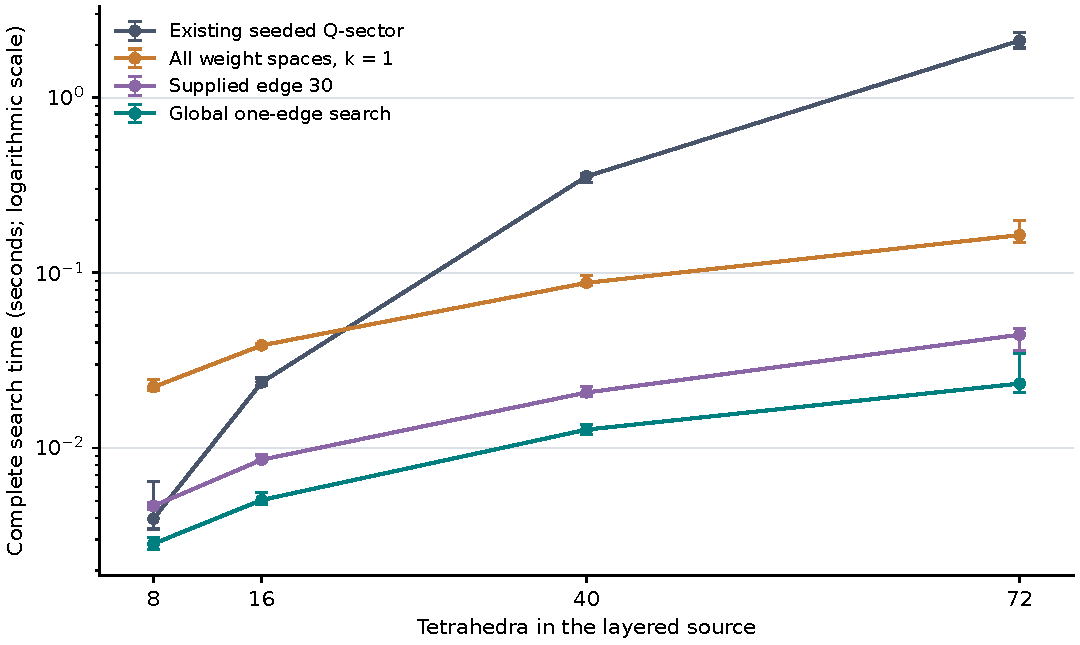
\includegraphics[width=.96\linewidth]{../artifacts/benchmark_plot.pdf}
\caption{Measured medians and full observed ranges on four structured
sources. The vertical axis is logarithmic. The lines connect measurements;
they are not fitted asymptotic laws. Source data and the plotting script
are supplied.}
\label{fig:benchmark}
\end{figure}

The supplied-edge arm includes preparation of its two-dimensional
arrangement, explaining why it is not necessarily faster than the
globally prepared sparse-incidence arm. Coherent-only search completes
quickly but finds no disc, so it is not included as a successful
recognition-time comparator.

On all four labelled fixtures, the global method begins 39 bases,
including the coherent attempt, and makes ten local tetrahedron
reconstructions before its one positive disc query. The deduplicated
global hyperplane counts are 72, 128, 296 and 520. These early-return
counters depend on the serialized edge ordering; the parameter and
completeness statement do not.

The existing seeded sector's matching nullity remains three throughout
the experiment. Its number of kernel variables grows through 16, 40,
112 and 208. The measured difference therefore reflects the amount and
organization of exact algebra and setup, rather than a growing sector
nullity. The elementary new all-subspace method is slower than the
existing solver on the two smallest sources; that unfavorable comparison
is retained. One family and four sizes do not establish a corpus-wide
speedup. The asymptotic theorem comes from the proofs above.

\subsection{Independent and adversarial verification}

The focused edge-discovery suite has 13 tests. It covers rational local
reconstruction, large binary coordinates, dependent coherent columns,
the old and new explicit discs, global caps, cancellation, input
immutability, and replay with corresponding producer functions disabled.

The polynomial vertex gate has seven supplementary tests, including
multiple boundary vertices, rejection of a vertex link with nonzero raw
parity but trivial cohomology class, nonextreme mixed surfaces, determinant
checks against direct small permutation sums, and forged certificates.
At 72 tetrahedra its supported minor has order 216. The compact
certificate has 2,789 bytes, excluding the separately supplied source and
normal vector; exact independent replay succeeds without an orbit query.

Regina independently enumerated 138 standard vertex surfaces across
eight triangulations of one through eight tetrahedra. Exact edge
reconstruction agrees on every vector. Twelve meridians satisfy the
signed/unsigned parity lower bound; eleven applicable subspace searches
recover their targeted standard vertex discs with cancellation support
at most two. The one-edge optimized search also succeeds whenever its
promise applies.

External topology checks confirm the layered family at
$r=0,1,2,4,8$. They are deliberately bounded by 10,000 normal pieces:
Regina's installed documentation states that the connectivity and
orientability methods used expand normal discs, and its compression
test may cut and retriangulate. An initial unrestricted large-family
external audit terminated with exit code 137; no conclusions use its
unretained partial results. The saved record explicitly marks omitted
external checks. Exact native binary certificates and supported-rank
checks remain in force at larger sizes, including the 72-tetrahedron
benchmark witness with more than $3\cdot10^{14}$ normal pieces.

The parallelity supplement's independent audit is described in
Section~\ref{sec:parallelity-interface}; it adds 184 literal geometric
comparisons, including 54 authenticated source comparisons, and huge
binary-coordinate replay. These tests measure different obligations
from vertex-disc discovery and are not added to its sample count.

The maintained suite contains 1,627 collected tests. Successful coverage
was reconciled across the initial broad run (1,512 successful tests) and a
115-test targeted rerun after restoring 20 historical dependency files
from the pinned revision. All 42 initial errors were missing-dependency
or setup errors, with no assertion failures; none remains unresolved.
Both logs, the restored-file list and the complete test identifiers are
included. The 13 new discovery tests are included in the maintained count;
the seven vertex-gate and eleven interface tests are additional.


These are exact-arithmetic programs and human-readable mathematical
proofs with independent review. They are not proof-assistant
formalizations. The principal residual mathematical obligation is the
source-coverage theorem, while the principal remaining implementation
obligations concern optimized general-$k$ enumeration and the transport
of boundary markings through actual geometric replacements.

\subsection{Package and integration procedure}

The archive contains the complete \LaTeX{} sources, compiled PDF,
figures, measurements, certificates, additive source overlay, a patch
against the pinned revision, and reproduction instructions. A small
baseline snapshot includes the dependencies needed by the focused
research experiments; it is not a replacement for the whole repository.

To integrate, first apply the additive discovery files to the pinned
source and run the focused suite. The interface and vertex-gate
supplements can be reviewed independently. Preserve the three trust
boundaries: a certified exterior source, a verified normal surface in
that source, and a justified coverage statement before turning finite
exhaustion into a global negative verdict. Broader default scheduling
should await a mixed-source benchmark that includes unfavorable cases,
relabellings, large-degree edges and preprocessing costs.
